\documentclass[aspectratio=169]{beamer}
\usepackage{lmodern}
\usepackage{beamerthemesplit}
\usepackage{multirow}
\usepackage{array}
\usepackage{hyperref}
\usepackage[T1]{fontenc}
\usepackage{inconsolata}
\usepackage{xcolor,colortbl}
\usepackage{natbib}
\usepackage{listings}
\usepackage{tikz}
\usepackage{graphicx}
\usetikzlibrary{matrix}
\let\Tiny\tiny
%%\newcommand{\newblock}{}
\DeclareGraphicsExtensions{.pdf,.png,.jpg}
\usetheme[pageofpages=of,% String used between the current page and the
                         % total page count.
          bullet=circle,% Use circles instead of squares for bullets.
          titleline=true,% Show a line below the frame title.
          alternativetitlepage=true,% Use the fancy title page.
          ]{Torino}
\definecolor{light-green}{RGB}{144,238,144}
\def\checkmark{\tikz\fill[scale=0.4](0,.35) -- (.25,0) -- (1,.7) -- (.25,.15) -- cycle;} 
\def\f{\textcolor{red}{x}}
\def\p{\textcolor{green}{\checkmark}}
\makeatletter
\setbeamertemplate{footline}
{
  \leavevmode%
  \hbox{%
  \begin{beamercolorbox}[wd=.333333\paperwidth,ht=2.25ex,dp=1ex,center]{author in head/foot}%
    \usebeamerfont{author in head/foot}\insertshortauthor~~\beamer@ifempty{\insertshortinstitute}{}{(\insertshortinstitute)}
  \end{beamercolorbox}%
  \begin{beamercolorbox}[wd=.333333\paperwidth,ht=2.25ex,dp=1ex,center]{title in head/foot}%
    \usebeamerfont{title in head/foot}\insertshorttitle
  \end{beamercolorbox}%
  \begin{beamercolorbox}[wd=.333333\paperwidth,ht=2.25ex,dp=1ex,right]{date in head/foot}%
    \usebeamerfont{date in head/foot}\insertshortdate{}\hspace*{2em}
%    \insertframenumber{} / \inserttotalframenumber\hspace*{2ex} % DELETED
  \end{beamercolorbox}}%
  \vskip0pt%
}
\makeatother
\begin{document}
\author{{\bf Casey Stella}}
\institute[Hortonworks]{
\includegraphics[width=80px,height=34px]{logo}}
\title{{\bf Streaming Outlier Analysis for Fun and Scalability}}
\date{2016} 

\frame{\titlepage} 

\frame{\frametitle{Table of Contents}\tableofcontents} 
\begingroup
\Huge
\begin{frame}
\frametitle{Introduction}
\begin{center}
Hi, I'm Casey Stella!
\end{center}
\end{frame}
\endgroup

\section{Streaming Analytics}
\begin{frame}
\frametitle{Streaming Analytics}
\begin{itemize}
\item The future involves non-trivial analytics done on streaming data
\item It's not just IoT
\item There is a need for insights to keep pace with the velocity of your data
\end{itemize}
\end{frame}

\begin{frame}
\frametitle{Streaming Analytics}
\begin{itemize}
\item {\textcolor{green}{\bf The Good:}} Much of the data can be coerced into timeseries\pause
\item {\textcolor{red}{\bf The Bad:}} There is a lot of data and it comes at you fast\pause
\item {\textcolor{green}{\bf The Good:}} Outlier analysis or anomaly detection is a killer-app\pause
\item {\textcolor{red}{\bf The Bad:}} Outlier analysis can be computationally intensive\pause
\item {\textcolor{green}{\bf The Good:}} There is no shortage of computational frameworks to handle streaming\pause
\item {\textcolor{red}{\bf The Bad:}} There are not an overabundance of high-quality outlier analysis frameworks
\end{itemize}
\end{frame}

\begin{frame}
\frametitle{Outlier Analysis}
Outlier analysis or anomaly detection is the analytical technique by which ``interesting'' points are differentiated from ``normal'' points.  Often ``interesting'' implies some sort of error or state which should be researched further.\pause
\\
Macrobase\footnote{http://arxiv.org/pdf/1603.00567v1.pdf}, an outlier analysis system built for IoT by MIT and Stanford and Cambridge Mobile Telematics, noted several properties of IoT data:
\begin{itemize}
\item Data produced by IoT applications often have come from some ``ordinary'' distribution
\item IoT anomalies are often systemic
\item They are often fairly rare
\end{itemize}
\end{frame}

\section{Framework}

\begin{frame}
\frametitle{Outlier Analysis: A Hybrid Approach}
In order to function at scale, a two-phase approach is taken
\begin{itemize}
\item For every data point\pause
  \begin{itemize}
  \item Detect outlier candidates using a robust estimator of variability (e.g. median absolute deviation) that uses distributional sketching (e.g. Q-trees)
  \item Gather a biased sample (biased by recency)\pause
  \item {\bf Extremely deterministic in space and cheap in computation}\pause
  \end{itemize}
\item For every outlier candidate
  \begin{itemize}
  \item Use traditional, more computationally complex approaches to outlier analysis (e.g. Robust PCA) on the biased sample\pause
  \item {\bf Expensive computationally, but run infrequently}\pause
  \end{itemize}
\end{itemize}
{\bf This becomes a data filter which can be attached to a timeseries 
data stream within a distributed computational framework (i.e. Storm, Spark, Flink, NiFi) to detect outliers.}
\end{frame}

\begin{frame}
\frametitle{Sketchy Outlier Estimator: Median Absolute Deviation}
\begin{itemize}
\item Median absolute deviation (or MAD) is a robust statistic\pause
  \begin{itemize}
  \item Robust statistics are statistics with good performance for data drawn from a wide range of non-normally distributed probability distributions
  \item Unlike the standard mean/standard deviation combo, MAD is not sensitive to the presence of outliers.\pause
  \end{itemize}
\item The median absolute deviation is defined for a series of univariate samples $X$ with $\tilde{x}=$median($X$), MAD($X$)=median(\{$\forall x_i \in X \lvert |x_i - \tilde{x}|$\}).\pause
\item A point is considered an outlier if its distance from the current window median, scaled by the MAD for the previous window, is above a threshold.\pause
\end{itemize}
{\bf tl;dr: A formal way to encode our intuition: If a point is far away from the ``central'' point of our window, then it's likely an outlier. }
\end{frame}

\begin{frame}
\frametitle{Architecture}
\begin{center}
  \makebox[\textwidth]{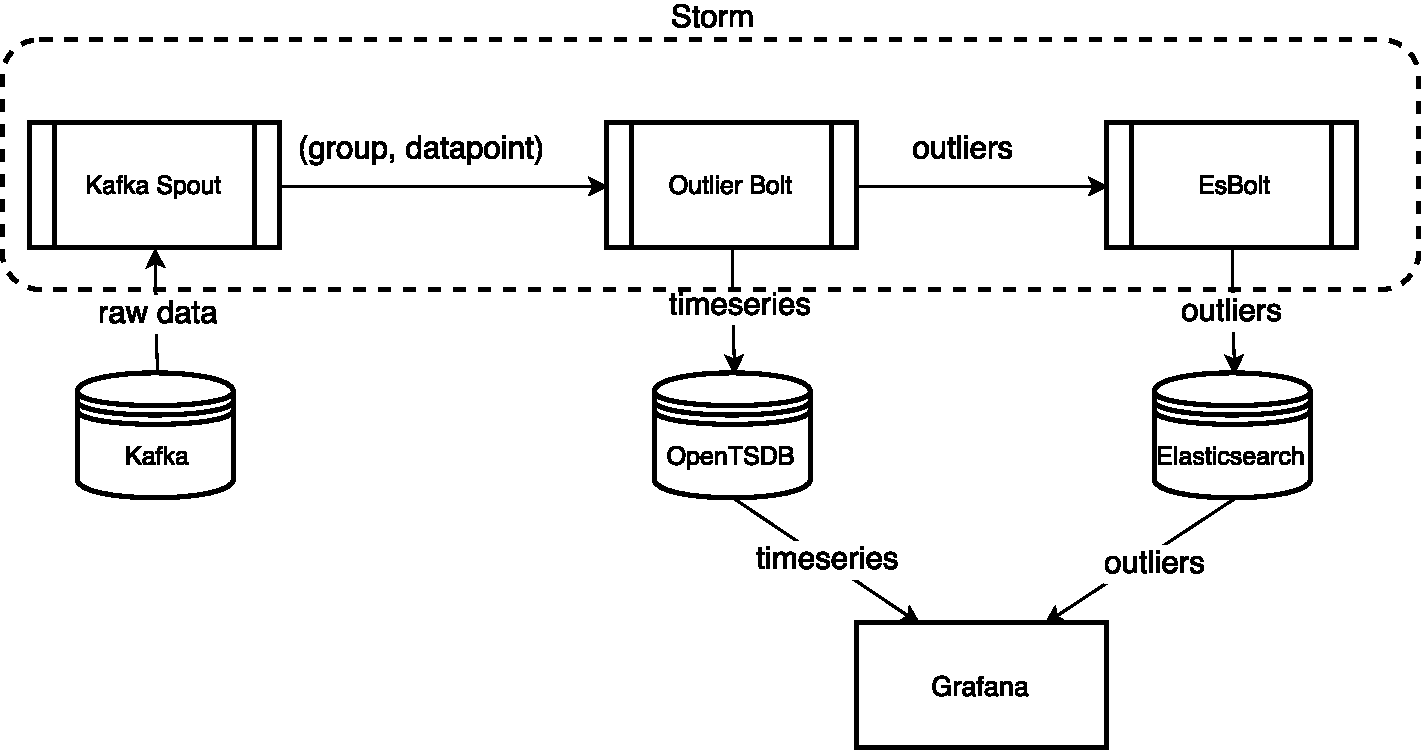
\includegraphics[scale=0.5]{images/streaming_outlier.pdf}}
\end{center}
\end{frame}


\section{Demos}
\begingroup
\Huge
\begin{frame}
\frametitle{Demos}
\begin{center}
Demos
\end{center}
\end{frame}
\endgroup


\section{Questions}

\frame{\frametitle{Questions}
Thanks for your attention!  Questions? 
\begin{itemize}
\item Code \& scripts for this talk available at http://github.com/cestella/streaming\_outliers
\item Find me at http://caseystella.com 
\item Twitter handle: @casey\_stella 
\item Email address: cstella@hortonworks.com
\end{itemize}
}


\end{document}
